%Este trabalho está licenciado sob a Licença Creative Commons Atribuição-CompartilhaIgual 4.0 Internacional. Para ver uma cópia desta licença, visite https://creativecommons.org/licenses/by-sa/4.0/ ou envie uma carta para Creative Commons, PO Box 1866, Mountain View, CA 94042, USA.

\chapter{Funções trigonométricas}
 Possivelmente seu primeiro contato com trigonometria, foi ao estudar a trigonometria no triângulo retângulo, neste caso definimos as funções trigonométricas como razões entre os lados do triângulo e estamos restringindo seu domínio aos ângulos entre $0 \degree$ e $90 \degree$.
 Quando a trigonometria aparece novamente nos currículos ela ressurge através do ciclo trigonométrico, que no começo fica restrito a compreensão da primeira volta do ciclo ou seja ângulos entre $0 \degree$ e $360 \degree$, para depois ainda sobre o ciclo aumentar o domínio da função.
 Antes de estudarmos as funções trigonométricas com domínio real vamos relembrar como este conceito era abordado nestes dois contextos já conhecidos.
 
 \section{Triângulo retângulo}

  Considere o triângulo retângulo, como na figura abaixo:
  % \begin{figure}[H]
  %  \centering
  %  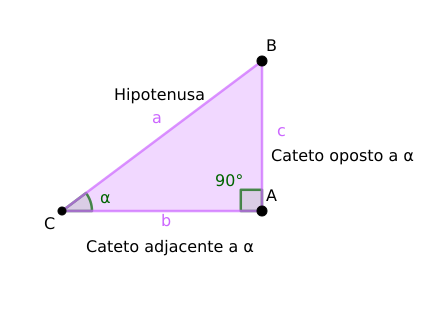
\includegraphics[width=7cm]{./cap_trigon/figs/triangulo_retangulo}
  % \end{figure}
  \begin{center}
  \begin{tikzpicture}[y=1cm]
    \draw (4,0) coordinate (A) -- (0,0) coordinate (B)
         -- (4,3) coordinate (C);
     \pic [draw, fill=gray!30, angle eccentricity=1.5] {angle};
     \pic [draw,fill=gray!30,thick,angle eccentricity=1]{right angle = B--A--C};
     \draw[draw=black] (0,0) node[anchor=north]{$B$}
      -- node[above] {$c$} node[sloped,below]{cateto adjacente} (4,0) node[anchor=north]{$A$}
      -- node[left] {$b$} node[sloped,below]{cateto oposto} (4,3) node[anchor=south]{$C$}
      -- node[sloped,below] {$a$} node[sloped,above]{hipotenusa} cycle;
      \draw (1,0) node[above left]{$\alpha$};
\end{tikzpicture}
  \end{center}
 para este triângulo temos que é válido o seguinte teorema:


\begin{teo}[Teorema de Pitágoras]
\begin{equation*}
  a^2= b^2 + c^2.
\end{equation*}
\end{teo}


 % \textit{Nota histórica:} De acordo com Howard Eves, em seu livro: \textit{"Introdução à história da Matemática"}, acredita-se que Pitágoras nasceu por volta de 572 a.c. na ilha egéia de Samos, e apesar deste teorema levar seu nome, este resultado já era conhecido pelos babilônios dos tempos de Hamurabi, mais de um milênio antes, mas sua primeira demonstração geral pode ter sido dada por Pitágoras.
 
 Este é um resultado importante, já que com ele é possível encontrar o valor de um dos lados do triângulo, nos casos em que não temos todos os lados dados.

 Para este triângulo, as funções seno, cosseno e tangente são dadas pelas seguintes razões trigonométricas, nesta ordem:
  \begin{align*}
   \sen(\alpha)&= \frac{c}{a}= \frac{\mbox{cateto oposto}}{\mbox{hipotenusa}} \ ; \\
   \cos(\alpha)&= \frac{b}{a}= \frac{\mbox{cateto adjacente}}{\mbox{hipotenusa}} \ ; \\
   \tg(\alpha)&= \frac{c}{b}= \frac{\mbox{cateto oposto}}{\mbox{cateto adjacente}}.
  \end{align*}
 
 Como a soma dos ângulos internos de um triângulo é $180 \degree$, e estamos aqui tratando de um triângulo retângulo, decorre que neste caso $0 \degree \leqslant \alpha \leqslant 90 \degree$. 
 
 Destacamos aqui os valores do seno, cosseno e tangente dos \emph{ângulos notáveis} que são os mais conhecidos:

 \begin{table}[H]
 \centering
 \begin{tabular}{|c|c|c|c|c|c|} \hline
 \rowcolor{gray}
               & $0 \degree$  & $30 \degree$  & $45 \degree$  & $60 \degree$ & $90 \degree$  \\\hline
  $\pmb{\sen}$ & $0$ &$\frac{1}{2}$ & $\frac{\sqrt{2}}{2}$ & $\frac{\sqrt{3}}{2}$ & $1$ \\\hline
  $\pmb{\cos}$ & $1$ & $\frac{\sqrt{3}}{2}$ & $\frac{\sqrt{2}}{2}$ & $\frac{1}{2}$ & $0$ \\\hline
  $\pmb{\tg}$ & $0$ & $\frac{\sqrt{3}}{3}$ & $1$ & $\sqrt{3}$ & $\nexists$ \\\hline
 \end{tabular}
\end{table}
 
 %Na próxima seção veremos como utilizar estes valores para calcular seno, cosseno e tangente de ângulos maiores que $90 \degree$.

 Os ângulos podem também ser representados em radianos, respeitando a seguinte relação:
  \destaque{\pi \text{ radianos}= 180 \degree}.

  Usando esta relação podemos transformar graus para radianos e radianos para graus, vamos ver dois exemplos:

  \begin{exem}
   Qual a medida em graus do ângulo que mede $\frac{\pi}{4}$ radianos?

   Sabemos que $\pi= 180\degree$, portanto usando a regra de 3 abaixo conseguimos encontrar o valor em graus deste ângulo:
   \begin{eqnarray*}
  \text{Graus} & & \text{Radianos} \\
   180 & = & \pi\\
  x & = & \frac{\pi}{4}
 \end{eqnarray*}
 usando a propriedade da proporcionalidade, ou seja, multiplicando cruzado temos:

 $180 \cdot \frac{\pi}{4}= \pi \cdot x \Rightarrow \pi \cdot x= \frac{180 \pi}{4} \Rightarrow x= \frac{45 \pi}{\pi} \Rightarrow x= 45\degree$.

 \fim
  \end{exem}

  \begin{exem}
   Qual a medida em radianos do ângulo que mede $30\degree$?

   Sabemos que $\pi= 180\degree$, portanto usando a regra de 3 abaixo conseguimos encontrar o valor em graus deste ângulo:
   \begin{eqnarray*}
  \text{Graus} & & \text{Radianos} \\
   180 & = & \pi\\
  30 & = & x
 \end{eqnarray*}
 usando a propriedade da proporcionalidade, ou seja, multiplicando cruzado temos:

 $180 \cdot x= \pi \cdot 30 \Rightarrow x= \frac{30 \pi}{180} \Rightarrow x= \frac{\pi}{6}$.

 \fim
  \end{exem}

Usualmente, denotaremos os ângulos em radianos. Desta forma podemos representar qualquer valor real de ângulo em radianos no ciclo trigonométrico.

\section{Ciclo trigonométrico}

Quando calculamos as relações trigonométricas no triângulo retângulo, estamos restrito à ângulos entre 0 e $90\degree$. O ciclo trigonométrico permite que calculemos seno, cosseno e tangente de qualquer valor real. Em geral, devemos usar ângulos em radianos.
 
 O ciclo trigonométrico é a circunferência de raio 1 com centro na origem associada à um sistema de coordenadas com as seguintes convenções:
 \begin{itemize}
     \item A origem $(0,0)$ é o centro da circunferência;
     \item O ponto $(1,0)$ é o ínicio de todos os arcos medidos;
     \item O sentido positivo do arco é anti-horário;
     \item A circunferência é dividida em quadro quadrantes.
 \end{itemize}
 
 \begin{figure}[H]
   \centering
   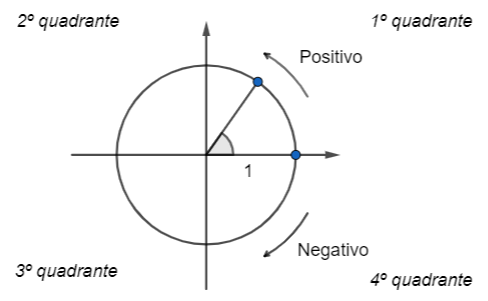
\includegraphics[width=7cm]
   {./cap_trigon/figs/ciclo_trogonometrico.png}
  \end{figure}

    Podemos associar a cada número real $x$ um ponto da circunferência trigonométrica considerando o arco de ângulo $x$ partindo do ponto $(1,0)$.

    Se o ponto da circunferência, final do arco iniciado 
 em $(1,0)$, é o mesmo para dois arcos diferentes, então chamamos estes arcos de arcos côngruos (ou congruentes). Observe que todos os arcos côngruos diferem si de um múltiplo de $2\pi$ rad (ou $360^\circ$), que é o comprimento de cada volta. Dessa forma, os arcos $x + 2k\pi$, para $k \in \Z$, são côngruos.

  %No plano cartesiano, consideremos um ciclo de centro na origem e raio $1$, neste ciclo representamos as imagens das funções trigonométricas aplicadas à  $x\in \R$ radianos.

\begin{obs}
    Dado $x \in\R$ com imagem de $x$ na circunferência trigonométrica sendo um ponto com coordenadas $(a,b)$, definimos:
    \begin{equation*}
        \cos x = a \ \mbox{ e } \sen x = b.
    \end{equation*}
\end{obs}

Dessa forma, passa-se a chamar o eixo das abscissas de eixo dos cossenos e o eixo das ordenadas de eixo dos senos, conforme no Geogrebra a seguir:

\geogebra{https://www.geogebra.org/m/cxrykpjv}{Seno, cosseno e tangente no ciclo trigonométrico}
  
 A figura mostra o ciclo trigonométrico para alguns ângulos notáveis:
 \begin{figure}[H]
   \centering
   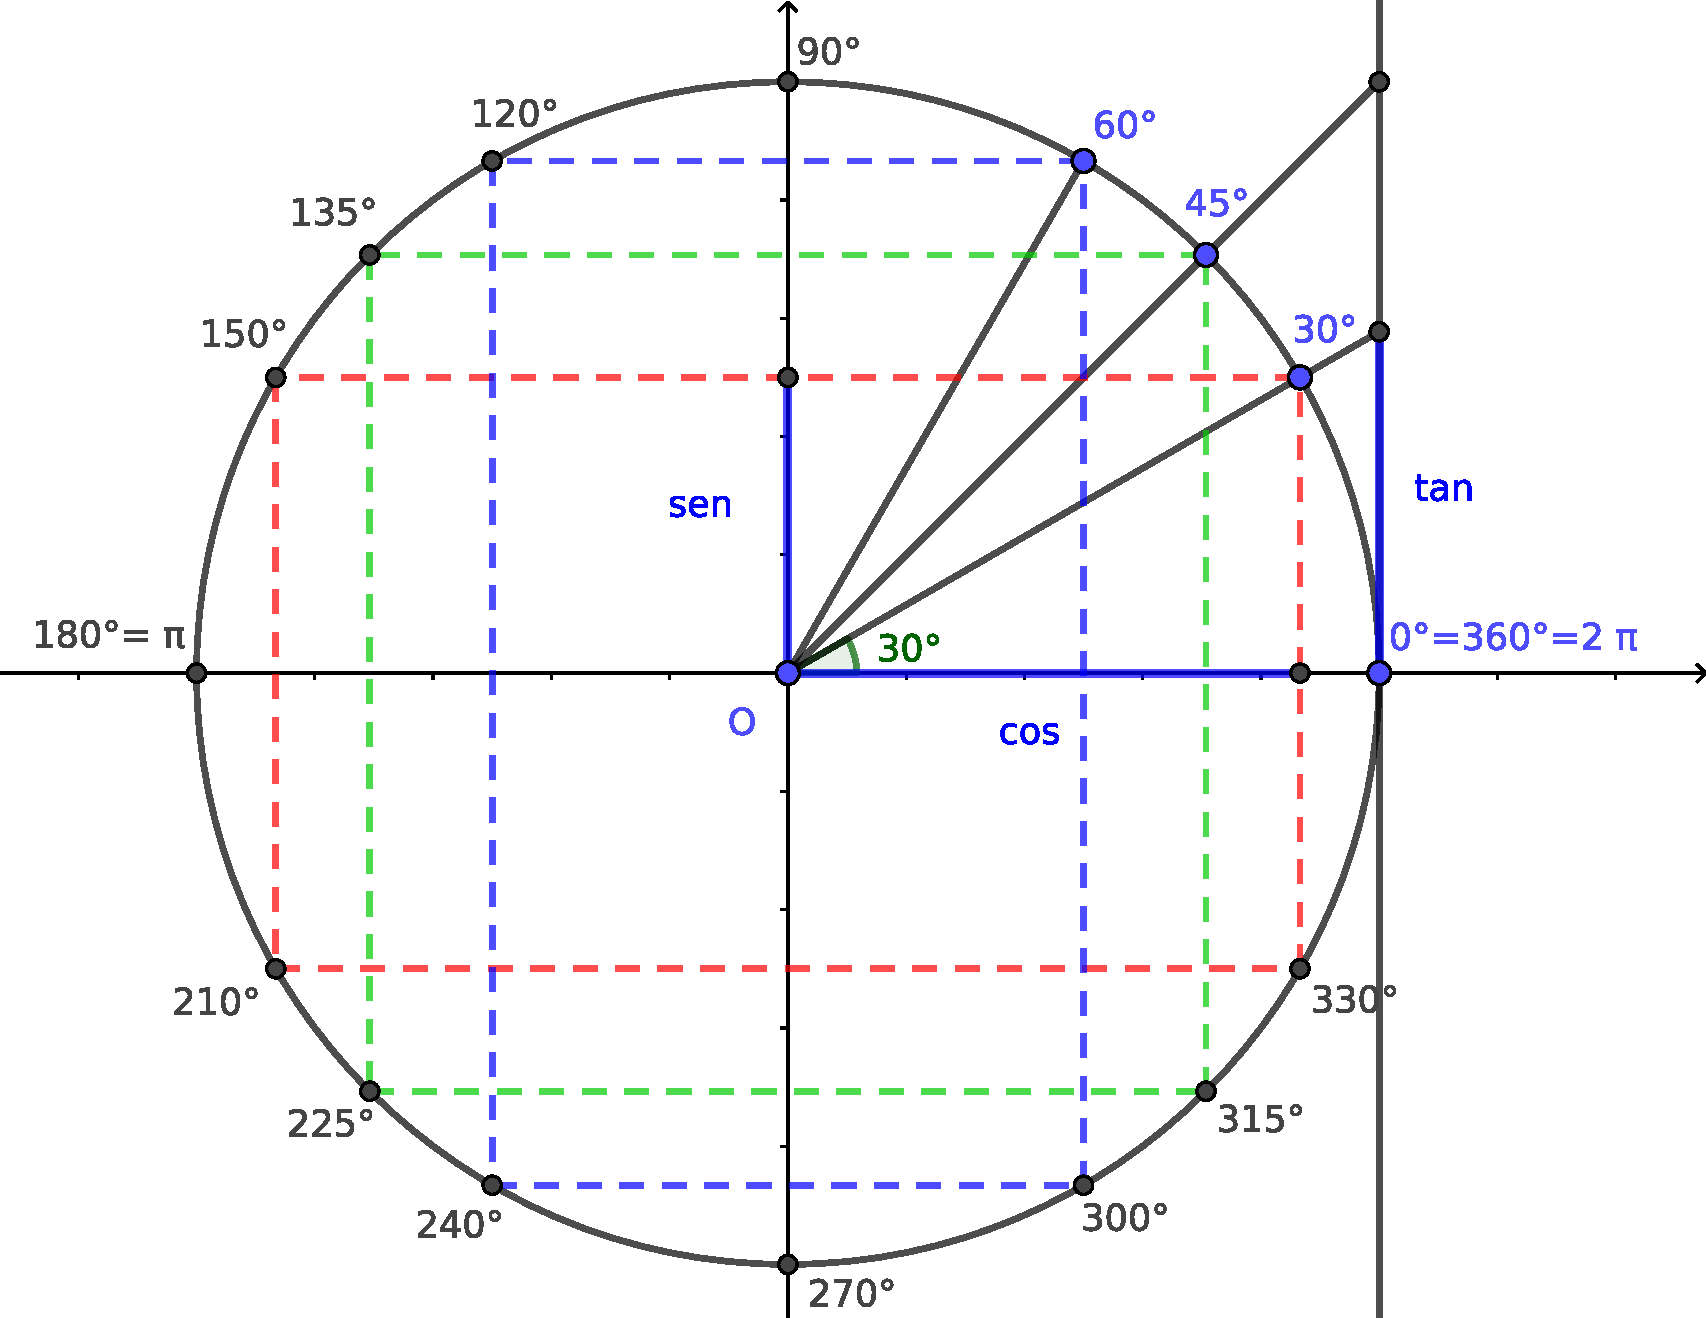
\includegraphics[width=9cm]{./cap_trigon/figs/circulo_trigonometrico}
  \end{figure}

 No ciclo trigonométrico acima, temos destacado o ângulo de $30 \degree$ formado pelo raio do ciclo com o eixo $x$. A projeção ortogonal deste raio sobre o eixo $x$ determina um segmento cujo comprimento é o valor do $\cos(30 \degree)$, sobre o eixo $y$ determina um segmento cujo comprimento é o valor do $\sen(30 \degree)$, e sobre a reta tangente determina um segmento cujo comprimento é o valor da $\tg(30 \degree)$. Podemos aqui trocar o ângulo de $30 \degree$ por qualquer outro valor e encontraremos os valores do cosseno, seno e tangente deste novo ângulo da mesma forma.



 
%   A partir do ciclo trigonométrico concluímos que:

%   \begin{table}[H]
%  \centering
%  \begin{tabular}{|c|c|c|c|} \hline
%  \rowcolor{gray}
%                &  $120\degree$  & $135\degree$  &  $150\degree$ \\\hline
%   $\pmb{\sen}$ & $\sen(60\degree)$ &$\sen(45\degree)$ & $\sen(30\degree)$  \\\hline
%   $\pmb{\cos}$ & $-\cos(60\degree)$ &$-\cos(45\degree)$ & $-\cos(30\degree)$  \\\hline
%   $\pmb{\tan}$ & $-\tan(60\degree)$ &$-\tan(45\degree)$ & $-\tan(30\degree)$  \\\hline
%  \end{tabular}
% \end{table}

%  \begin{table}[H]
%  \centering
%  \begin{tabular}{|c|c|c|c|} \hline
%  \rowcolor{gray}
%                 & $210\degree$ & $225\degree$  & $240\degree$  \\\hline
%   $\pmb{\sen}$ &  $-\sen(30\degree)$ & $-\sen(45\degree)$ & $-\sen(60\degree)$  \\\hline
%   $\pmb{\cos}$ &  $-\cos(30\degree)$ & $-\cos(45\degree)$ & $-\cos(60\degree)$  \\\hline
%   $\pmb{\tan}$ &  $\tan(30\degree)$ & $\tan(45\degree)$ & $\tan(60\degree)$   \\\hline
%  \end{tabular}
% \end{table}

%  \begin{table}[H]
%  \centering
%  \begin{tabular}{|c|c|c|c|} \hline
%  \rowcolor{gray}
%                & $300\degree$ & $315\degree$ & $330\degree$ \\\hline
%   $\pmb{\sen}$ & $\sen(60\degree)$ & $\sen(45\degree)$ & $\sen(30\degree)$ \\\hline
%   $\pmb{\cos}$ & $\cos(60\degree)$ & $\cos(45\degree)$ & $\cos(30\degree)$  \\\hline
%   $\pmb{\tan}$ & $-\tan(60\degree)$ & $-\tan(45\degree)$ & $-\tan(30\degree)$  \\\hline
%  \end{tabular}
% \end{table}


\begin{obs}
    \textbf{Identidade fundamental:} Para qualquer valor real $x\in \R$, temos que
    \begin{equation*}
        \sen^2 x +\cos^2 x = 1.
    \end{equation*}
\end{obs}


%\begin{secExercicios}

%\subsection*{Respostas}

%\shipoutAnswer

%\end{secExercicios}

\section{Funções trigonométricas}
   
 Vamos agora definir as funções trigonométricas no maior subconjunto real possível, e estudar o comportamento de seus gráficos. Mas para que este estudo seja completo precisamos antes definir os conceitos de período e amplitudade que são particularmente utéis para a compreenssão das funções trigonométricas.
 
  Estas funções fazem parte do grupo de funções periódicas, que são as funções que satisfazem a seguinte definição.

  \begin{obs}
   Uma função real $f: R \rightarrow \R$ é denominada \emph{periódica} quando existe um número real positivo $P$ tal que
\begin{equation*}
f(x + P)= f(x)
\end{equation*}
   para todo $x$ no domínio da $f$. O menor número real positivo $P$ que satisfaz esta propriedade é denominado período de $f$.
  \end{obs}
  
  Assim para entender seu comportamento em $\R$ basta conhecer como ela se comporta em um período.
  
  Além de periódica algumas funções trigonométricas são limitadas, ou seja admitem um valor máximo e um valor mínimo, e para estas funções podemos definir o conceito de amplitude como segue.
  
  \begin{obs}
  A \emph{amplitude} de oscilação $A$ de uma função limitada é dada por
  \begin{equation*}
  A= \frac{y_{max} - y_{min}}{2} .
  \end{equation*}
  \end{obs}
  
  De posse deste conceitos passamos agora para a definição das funções trigonométricas.
  
  \begin{itemize}
  \item \textbf{Função Seno:} $f: \R \rightarrow \R$ dada por $f(x)= \sen (x)$, cujo gráfico é:

  \begin{figure}[H]
  \centering
    \fbox{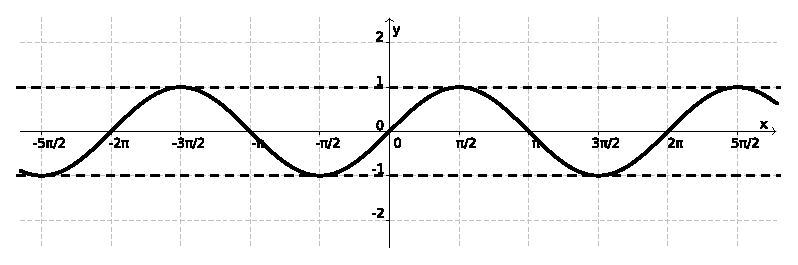
\includegraphics[width=10cm]{./cap_trigon/figs/sen}}
    \caption{Gráfico da função $f(x)= \sen(x)$}
  \end{figure}

%  A função seno tem período $2\pi$, amplitude $1$ e imagem $[-1,1]$.

  \item \textbf{Função Cosseno:} $f: \R \rightarrow [-1, 1]$ dada por $f(x)= \cos(x)$, cujo gráfico é:

  \begin{figure}[H]
  \centering
    \fbox{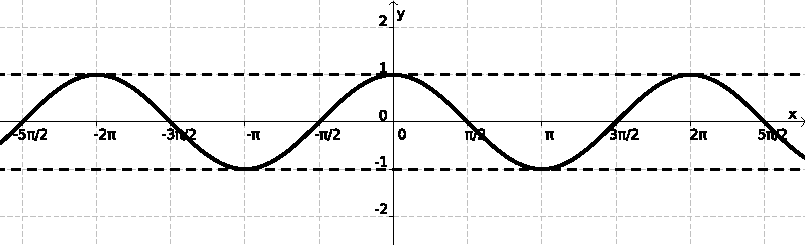
\includegraphics[width=10cm]{./cap_trigon/figs/cos}}
    \caption{Gráfico da função $f(x)= \cos(x)$}
  \end{figure}

  Geometricamente podemos observar que o comportamento do gráfico das funções seno o cosseno no intervalo $[0, 2\pi]$ se repete em cada intervalo de comprimento $2\pi$. Isso pode ser visualizado também olhando para o ciclo trigonométrico, por exemplo quando estamos olhando para um ângulo $\theta= 4\pi + \frac{\pi}{4}$ estamos apenas dando duas voltas no ciclo trigonométrico e andando mais $\frac{\pi}{4}$, por isso:
\begin{equation*}
\sen(4\pi + \frac{\pi}{4})= \sen(\frac{\pi}{4}) ,
\end{equation*}
\begin{equation*}
\cos(4\pi + \frac{\pi}{4})= \cos(\frac{\pi}{4}). 
\end{equation*}
  
  Funções com esta propriedade de repetição de comportamento são denominadas funções periódicas, e o intervalo que se repete é chamado de período.  Por interpretação do ciclo trigonométrico vemos que, para todo $x \in \R$:
\begin{equation*}
\sen(x + 2 \pi)= \sen(x) ,
\end{equation*}
\begin{equation*}
\cos(x + 2\pi)= \cos(x). 
\end{equation*}
  
  Logo as funções seno e cosseno são de fato funções períodicas de período $2\pi$.
  
  Além disso note que ambas as funções seno e cosseno são limitadas, com $y_{max}= 1$ e $y_{min}= -1$, portanto para ambas temos sua amplitude será:
  \begin{equation*}
  A= \frac{y_{max} - y_{min}}{2}= \frac{1 - (-1)}{2}= \frac{1+1}{2}= 1.
  \end{equation*}
  
  Para as demais funções trigonométricas que apresentaremos a seguir, convidamos o leitor a observar que elas não são limitadas e por este motivo não faz sentido falar de amplitudade para estas funções.

  \item \textbf{Função Tangente:} $f: \{x\in\R \colon \frac{\pi}{2} +k\pi, \mbox{ com } k \in \Z\} \rightarrow \R$ dada por
  \begin{equation*}
      f(x)= \tg(x) = \frac{\sen x}{\cos x},
  \end{equation*}
    cujo gráfico é:

  \begin{figure}[H]
  \centering
    \fbox{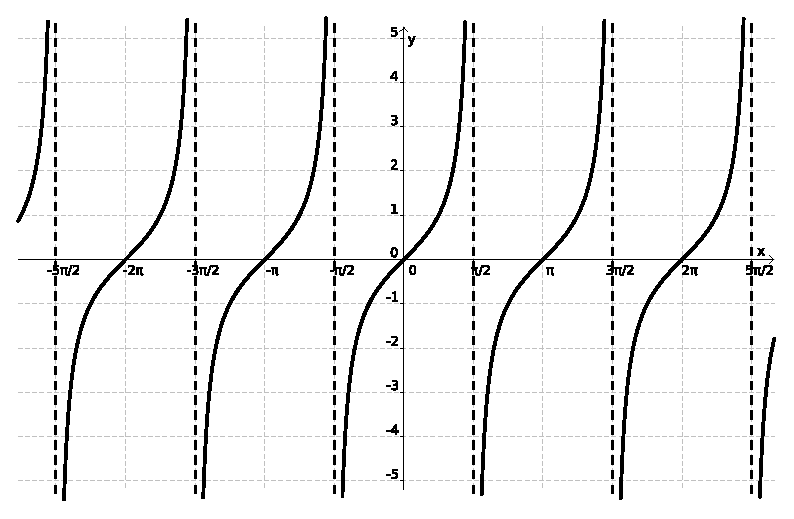
\includegraphics[width=10cm]{./cap_trigon/figs/tan}}
    \caption{Gráfico da função $f(x)= \tg (x)$}
  \end{figure}

  Podemos entender o domínio da função tangente como o conjunto dos $x \in \R$ tais que $\cos(x) \neq 0$.

  Note que o comportamento do gráfico da função tangente no intervalo $(-\frac{\pi}{2}, \frac{\pi}{2})$ se repete indefinadamente, e ainda
\begin{equation*}
\tg(x)= \tg(x + \pi)
\end{equation*}
  donde concluímos que a função tangente é uma função períodica de período $\pi$.

    \item \textbf{Função Cotangente:} $f: \{x\in\R \colon k\pi, \mbox{ com } k \in \Z\} \rightarrow \R$ dada por 
    \begin{equation*}
    f(x)= \cotg(x) = \frac{\cos x}{\sen x},
    \end{equation*}
    cujo gráfico é:

  \begin{figure}[H]
  \centering
    \fbox{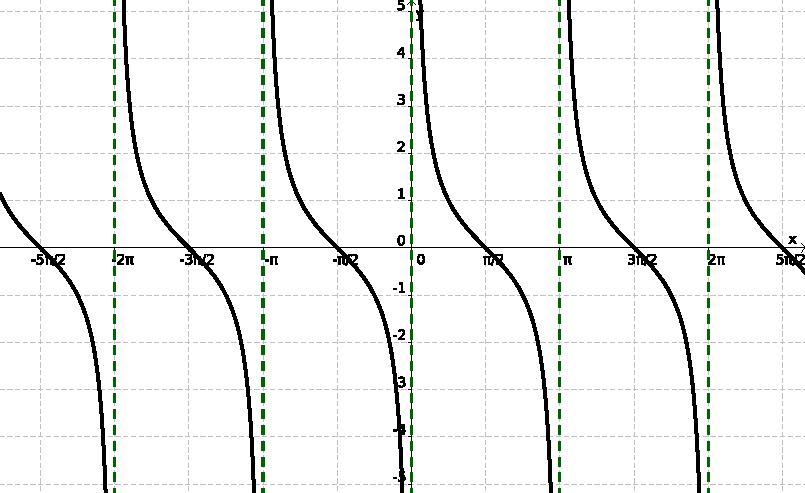
\includegraphics[width=10cm]{./cap_trigon/figs/cot}}
    \caption{Gráfico da função $f(x)= \cotg(x)$}
  \end{figure}

  O domínio da função cotangente é o conjunto dos $x \in \R$ tais que $\sen(x) \neq 0$.

  Já no gráfico da função cotangente vemos a repetição do comportamento do intervalo $(0, \pi)$, e temos que
\begin{equation*}
\cotg(x + \pi)= \cotg(x)
\end{equation*}
  portanto esta é uma função periódica de período $\pi$.
  

 \item \textbf{Função Secante:} $f: \{x\in\R \colon \frac{\pi}{2} +k\pi, \mbox{ com } k \in \Z\} \rightarrow \R$ dada por
  \begin{equation*}
      f(x)= \sec(x) = \frac{1}{\cos x},
  \end{equation*}
    cujo gráfico é:

  \begin{figure}[H]
  \centering
    \fbox{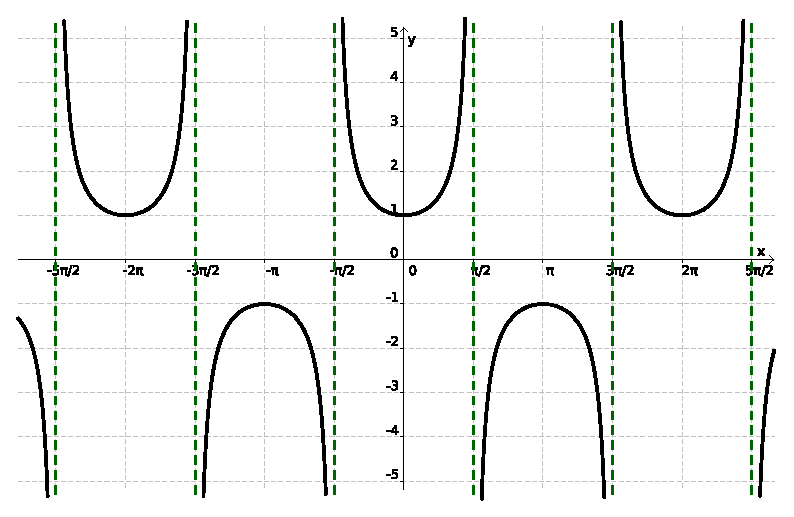
\includegraphics[width=10cm]{./cap_trigon/figs/sec}}
    \caption{Gráfico da função $f(x)= \sec(x)$}
  \end{figure}

  Como $\sec(x)= \dfrac{1}{\cos (x)}$ o domínio da função secante é o conjunto dos $x \in \R$ tais que $\cos(x) \neq 0$.

  Ao observar o gráfico da função secante notamos que o intervalo que se repete neste caso é $(\frac{-\pi}{2}, \frac{\pi}{2}) \cup (\frac{\pi}{2}, \frac{3\pi}{2})$, e ainda que
\begin{equation*}
\sec(x + 2\pi)= \sec(x) \ ,
\end{equation*}
  logo esta é uma função periódica com período $2\pi$.
  
  \item \textbf{Função Cossecante:} $f: \{x\in\R \colon k\pi, \mbox{ com } k \in \Z\} \rightarrow \R$ dada por 
    \begin{equation*}
    f(x)= \cossec(x) = \frac{1}{\sen x},
    \end{equation*}
    cujo gráfico é:

  \begin{figure}[H]
  \centering
    \fbox{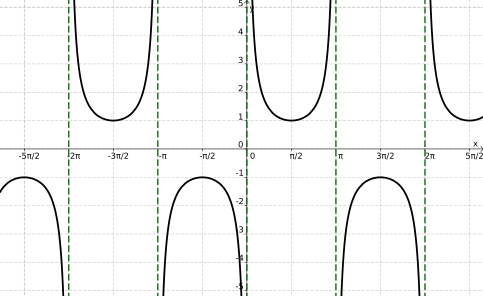
\includegraphics[width=10cm]{./cap_trigon/figs/csc}}
    \caption{Gráfico da função $f(x)= \cossec(x)$}
  \end{figure}

  Como $\csc(x)= \dfrac{1}{\sen(x)}$ o domínio da função cossecante é exatamente o conjunto dos $x \in \R$ tais que $\sen(x) \neq 0$.

  Ao observar o gráfico da função cossecante notamos que o gráfico da função no intervalo $(0, \pi) \cup (\pi, 2 \pi)$ se repete indefinidamente, e ainda
\begin{equation*}
\cossec(x + 2\pi)= \cossec(x) \ , 
\end{equation*}
  logo esta é uma função periódica, com período $2\pi$.

\end{itemize}
    
  \subsection{Funções Inversas}

  As funções trigonométricas admitem inversas quando restringimos seus domínios e contradomínios de forma a torná-las bijetoras, assim temos por exemplo as seguintes funções:

\begin{itemize}
  \item \textbf{Função Arco Seno:} $f: [-1, 1] \rightarrow [\frac{-\pi}{2}, \frac{\pi}{2}]$ dada por $f(x)= \arcsen(x)$. Neste caso o gráfico será:

  \begin{figure}[H]
  \centering
    \fbox{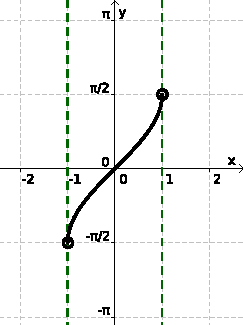
\includegraphics[width=5cm]{./cap_trigon/figs/arcsen}}
    \caption{Gráfico da função $f(x)= \arcsen(x)$}
  \end{figure}


  \item \textbf{Função Arco Cosseno:} $f: [-1, 1] \rightarrow [0, \pi]$ dada por $f(x)= \arccos(x)$. Neste caso temos o seguinte gráfico:

  \begin{figure}[H]
  \centering
    \fbox{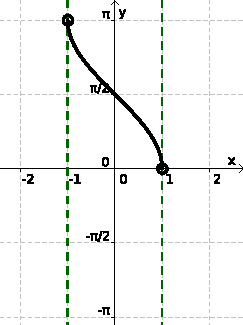
\includegraphics[width=5cm]{./cap_trigon/figs/arccos}}
    \caption{Gráfico da função $f(x)= \arccos(x)$}
  \end{figure}


  \item \textbf{Função Arco Tangente:} $f: \R \rightarrow (\frac{-\pi}{2}, \frac{\pi}{2})$, dada por $f(x)= \arctg(x)$. Neste caso o gráfico será:

  \begin{figure}[H]
  \centering
    \fbox{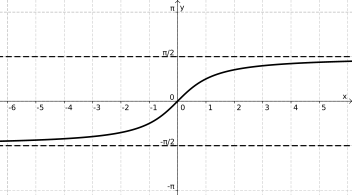
\includegraphics[width=10cm]{./cap_trigon/figs/arctan}}
    \caption{Gráfico da função $f(x)= \arctg(x)$}
  \end{figure}


  \end{itemize}

\section{Identidades trigonométricas}

 Nesta seção exibiremos algumas fórmulas útil no estudo de funções trigonométricas:
 
\vspace{.5cm}
 \textbf{Identidades de quociente:}
\begin{align*}
\tg(x) &= \dfrac{\sen(x)}{\cos(x)}; & \cotg(x) &= \dfrac{\cos(x)}{\sen(x)}.
\end{align*}

 \textbf{Identidades recíprocas:}
\begin{align*}
\sec(x) &= \dfrac{1}{\cos(x)}; &
   \cossec(x)&= \dfrac{1}{\sen(x)}; &
   \cotg(x)&= \dfrac{1}{\tan(x)}.  
\end{align*}

 \textbf{Identidades pitagóricas:}
\begin{align*}
    \sen^2(x) + \cos^2(x) &= 1; &
   \tg^2(x)+ 1 &= \sec^2(x); &
   \cotg^2(x)+1 &=\cossec^2(x).
\end{align*}

 \textbf{Identidades associadas à paridade:}

\begin{align*}
\sen(-x)&= -\sen(x);
& \cos(-x)&= \cos(x);&
\tg(-x)&=-\tg(x).
\end{align*}

 \textbf{Identidades de arcos complementares:}
\begin{align*}
    \sen \left(\frac{\pi}{2} - x \right) &= \cos(x); & \cos \left(\frac{\pi}{2} - x \right) &= \sen(x); \\
    \tg \left(\frac{\pi}{2} - x \right) &= \cotg(x); &
    \cotg \left(\frac{\pi}{2} - x \right) &= \tg(x);\\
    \cossec \left(\frac{\pi}{2} - x \right) &= \sec(x); &
   \sec \left(\frac{\pi}{2} - x \right) &= \cossec(x).
\end{align*}

 \textbf{Fórmulas de adição e subtração:}
 \begin{align*}
  \sen(a\pm b)&=\sen(a)\cdot \cos(b)\pm\sen(b)\cdot \cos(a); \\
  %\sen(a-b)&=\sen(a)\cdot \cos(b)-\sen(b)\cdot \cos(a);\\ 
  \cos(a\pm b)&=\cos(a)\cdot \cos(b)\mp\sen(a)\cdot \sen(b); \\
  %\cos(a-b)&=\cos(a)\cdot \cos(b)+\sen(a)\cdot \sen(b);\\ \\
  \tg(a\pm b)&= \frac{\tg(a)\pm\tg(b)}{1-\tg(a)\cdot \tg(b)};
  %\tan(a-b)&= \frac{\tan(a)-\tan(b)}{1-\tan(a)\cdot \tan(b)}.
 \end{align*}


\begin{secExercicios}

\begin{exer}
Expresse:
\begin{enumerate}[a)]
\begin{multicols}{2}
    \item 60º em radianos.
    \item 210º em radianos.
    \item 270º em radianos.
    \item $\frac{10\pi}{9}$ em graus.
    \item $\frac{\pi}{20}$ em graus.
    \item $\frac{3\pi}{4}$ em graus. 
\end{multicols}   
\end{enumerate}
\end{exer}

\begin{exer}
Represente no ciclo trigonométrico e calcule:
\begin{multicols}{2}
\begin{enumerate}[a)]
\item $\cos\left(\dfrac{9\pi}{4}\right)$
\item $\sen\left(-\dfrac{2\pi}{3}\right)$
\item $\sen\left(\dfrac{7\pi}{6}\right)$
\item $\cos\left(-\dfrac{11\pi}{2}\right)$
\item $\tg\left(\dfrac{3\pi}{4}\right)$
\item $\arcsen\left(-\dfrac{\sqrt{3}}{2}\right)$
\item $\arccos\left(\dfrac{1}{2}\right)$
\item $\arctg\left(-1\right)$
\end{enumerate}
\end{multicols}    
\end{exer}

\begin{exer}
    Esboce o gráfico e determine a imagem e o período das funções a seguir:
    \begin{enumerate}[a)]
        \item $f(x)=3\sen(\frac{x}{2})$
        \item $f(x)=2\sen x-3$
        \item $f(x)=\frac{1}{4}\cos(2x-\frac{\pi}{4})$
        \item $f(x)=2+\cos x$
        \item $f(x)=2\tg(x-\frac{\pi}{4})$
        \item $f(x)=-1+\tg(\frac{x}{3})$
        \item $f(x)=-\tg(2x)$
        \item $f(x)=3\sec(2x+\frac{\pi}{3})$
        \item $f(x)=|\sen x|$
        \item $f(x)=|\cos x|$
        \item $f(x)=|\tg x|$, para $x\in(-\frac{\pi}{2}, \frac{\pi}{2})$
    \end{enumerate}
\end{exer}

\begin{exer}
    Indique um tranformação de uma função trigonométrica para os gráficos a seguir, justificando sua resposta:

    \begin{center}
        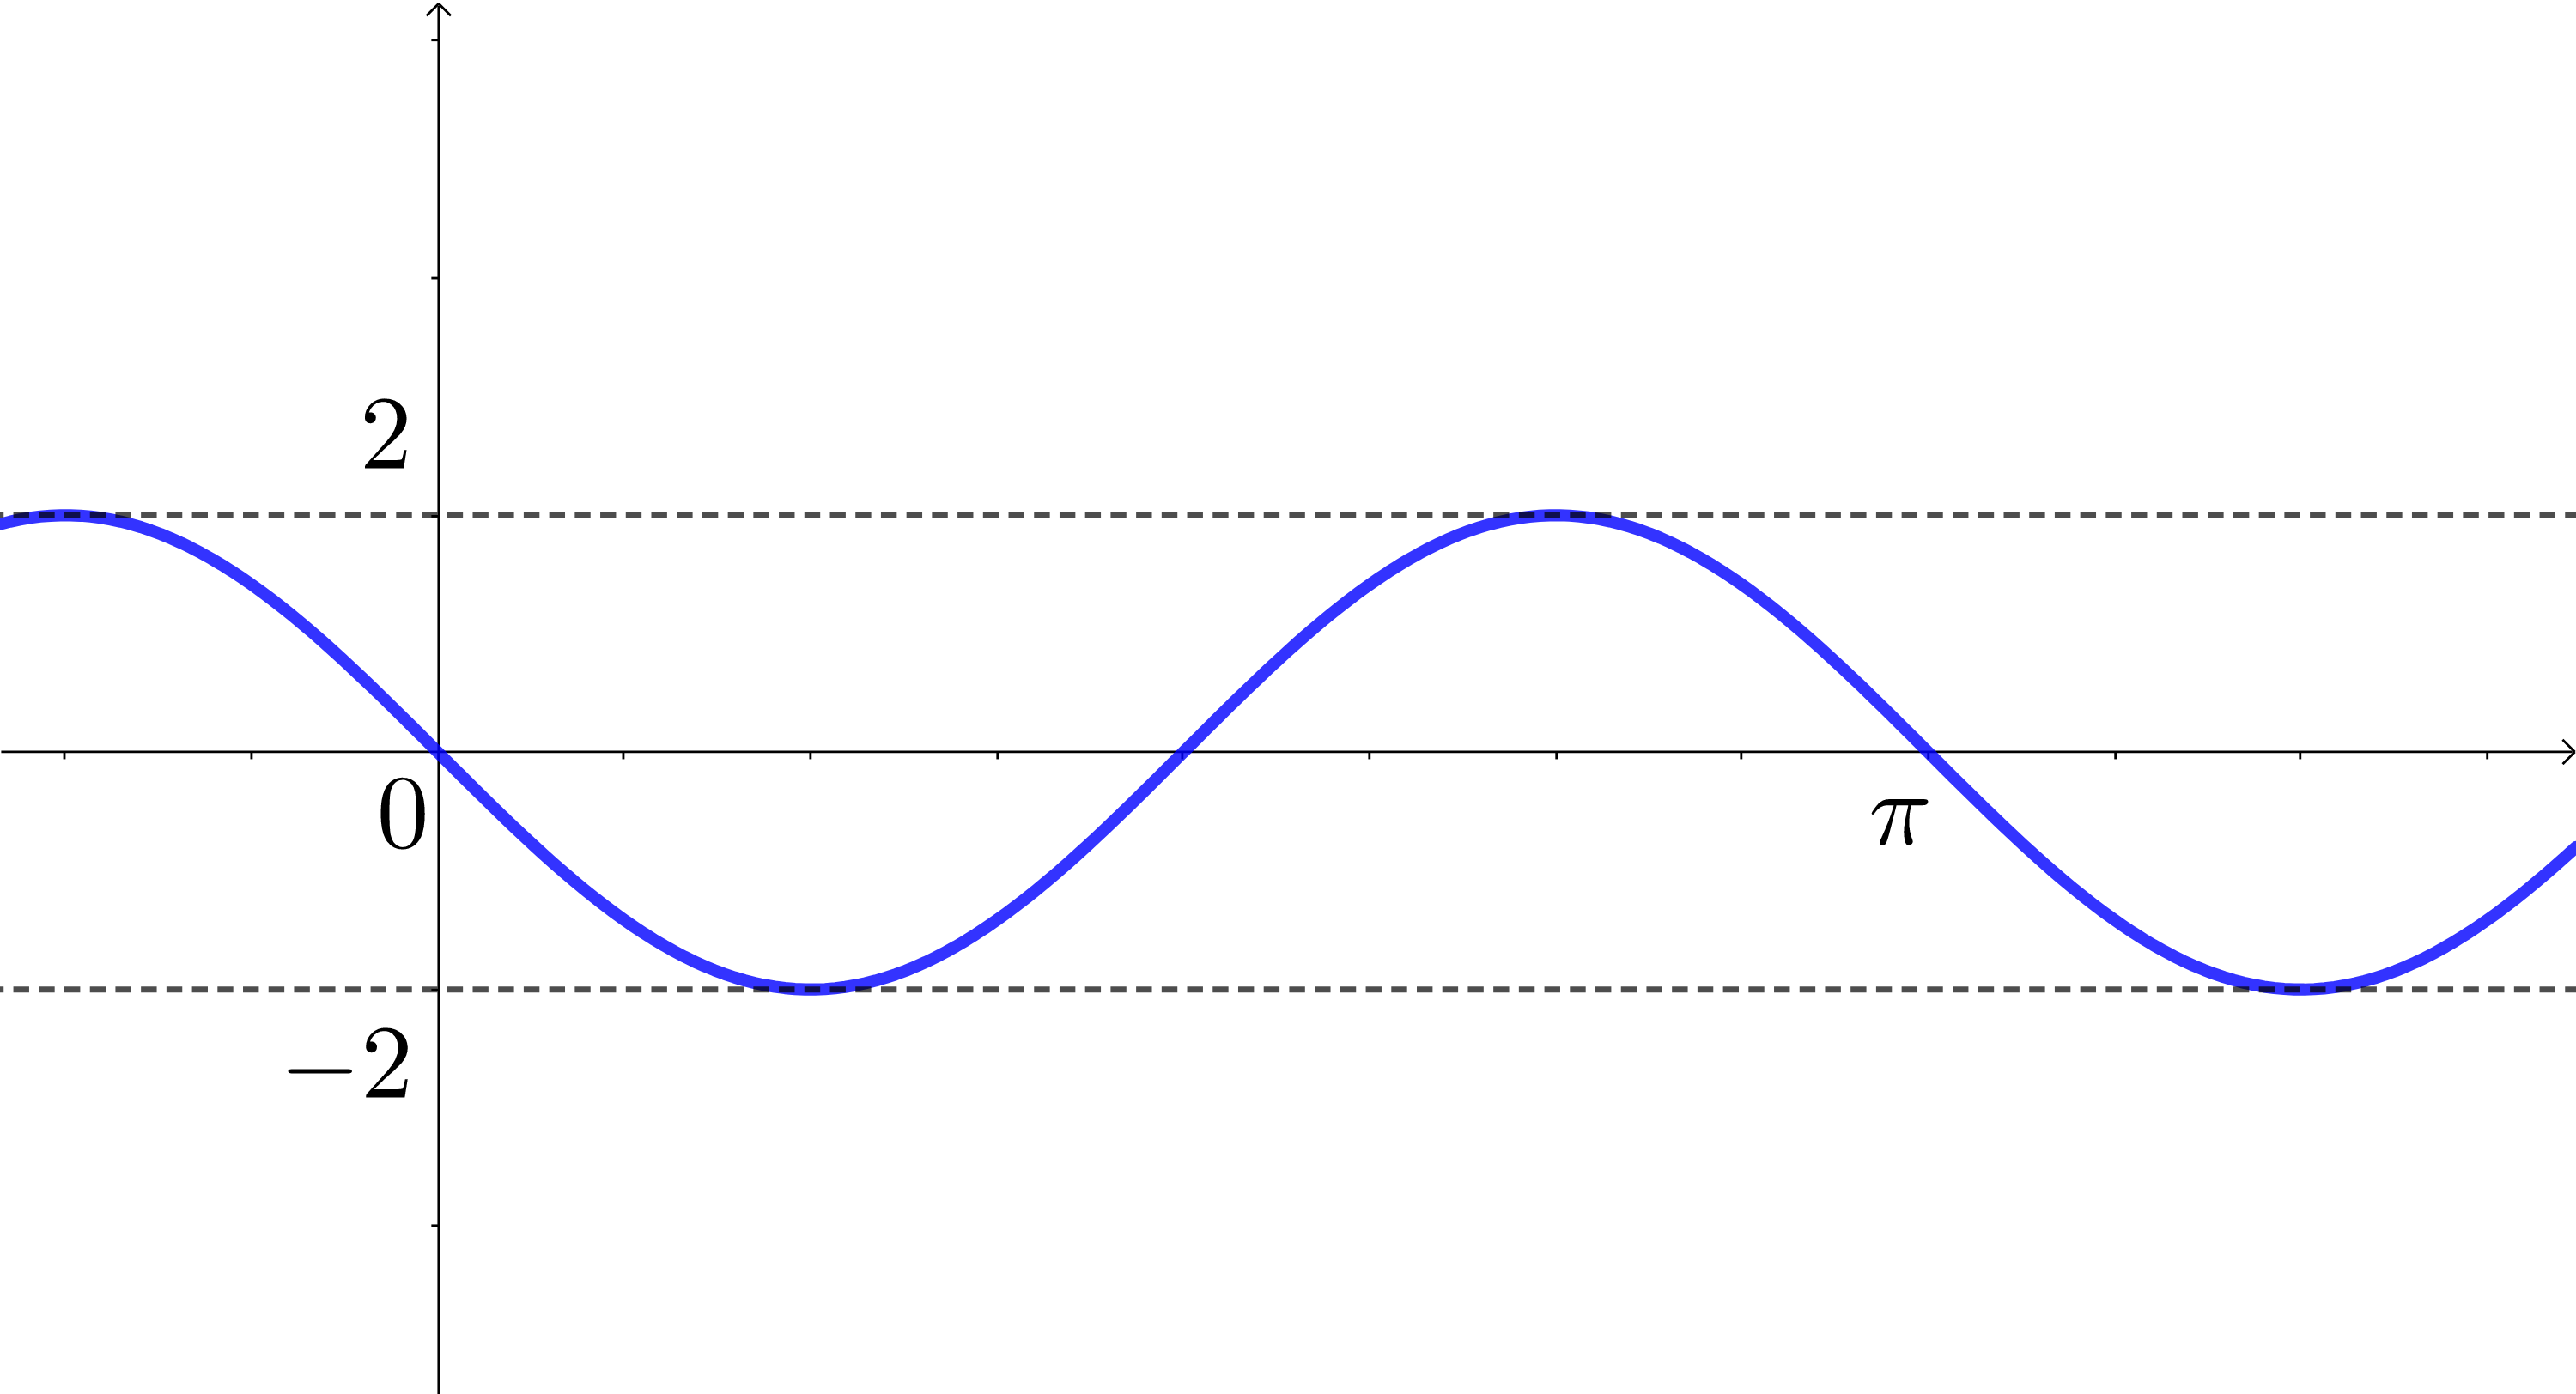
\includegraphics[width=6cm]{cap_trigon/figs/Grafico4.png}
        \vspace{.3cm}
        
        \includegraphics[width=6cm]{cap_trigon/figs/Grafico1.png}
        \vspace{.3cm}
        
        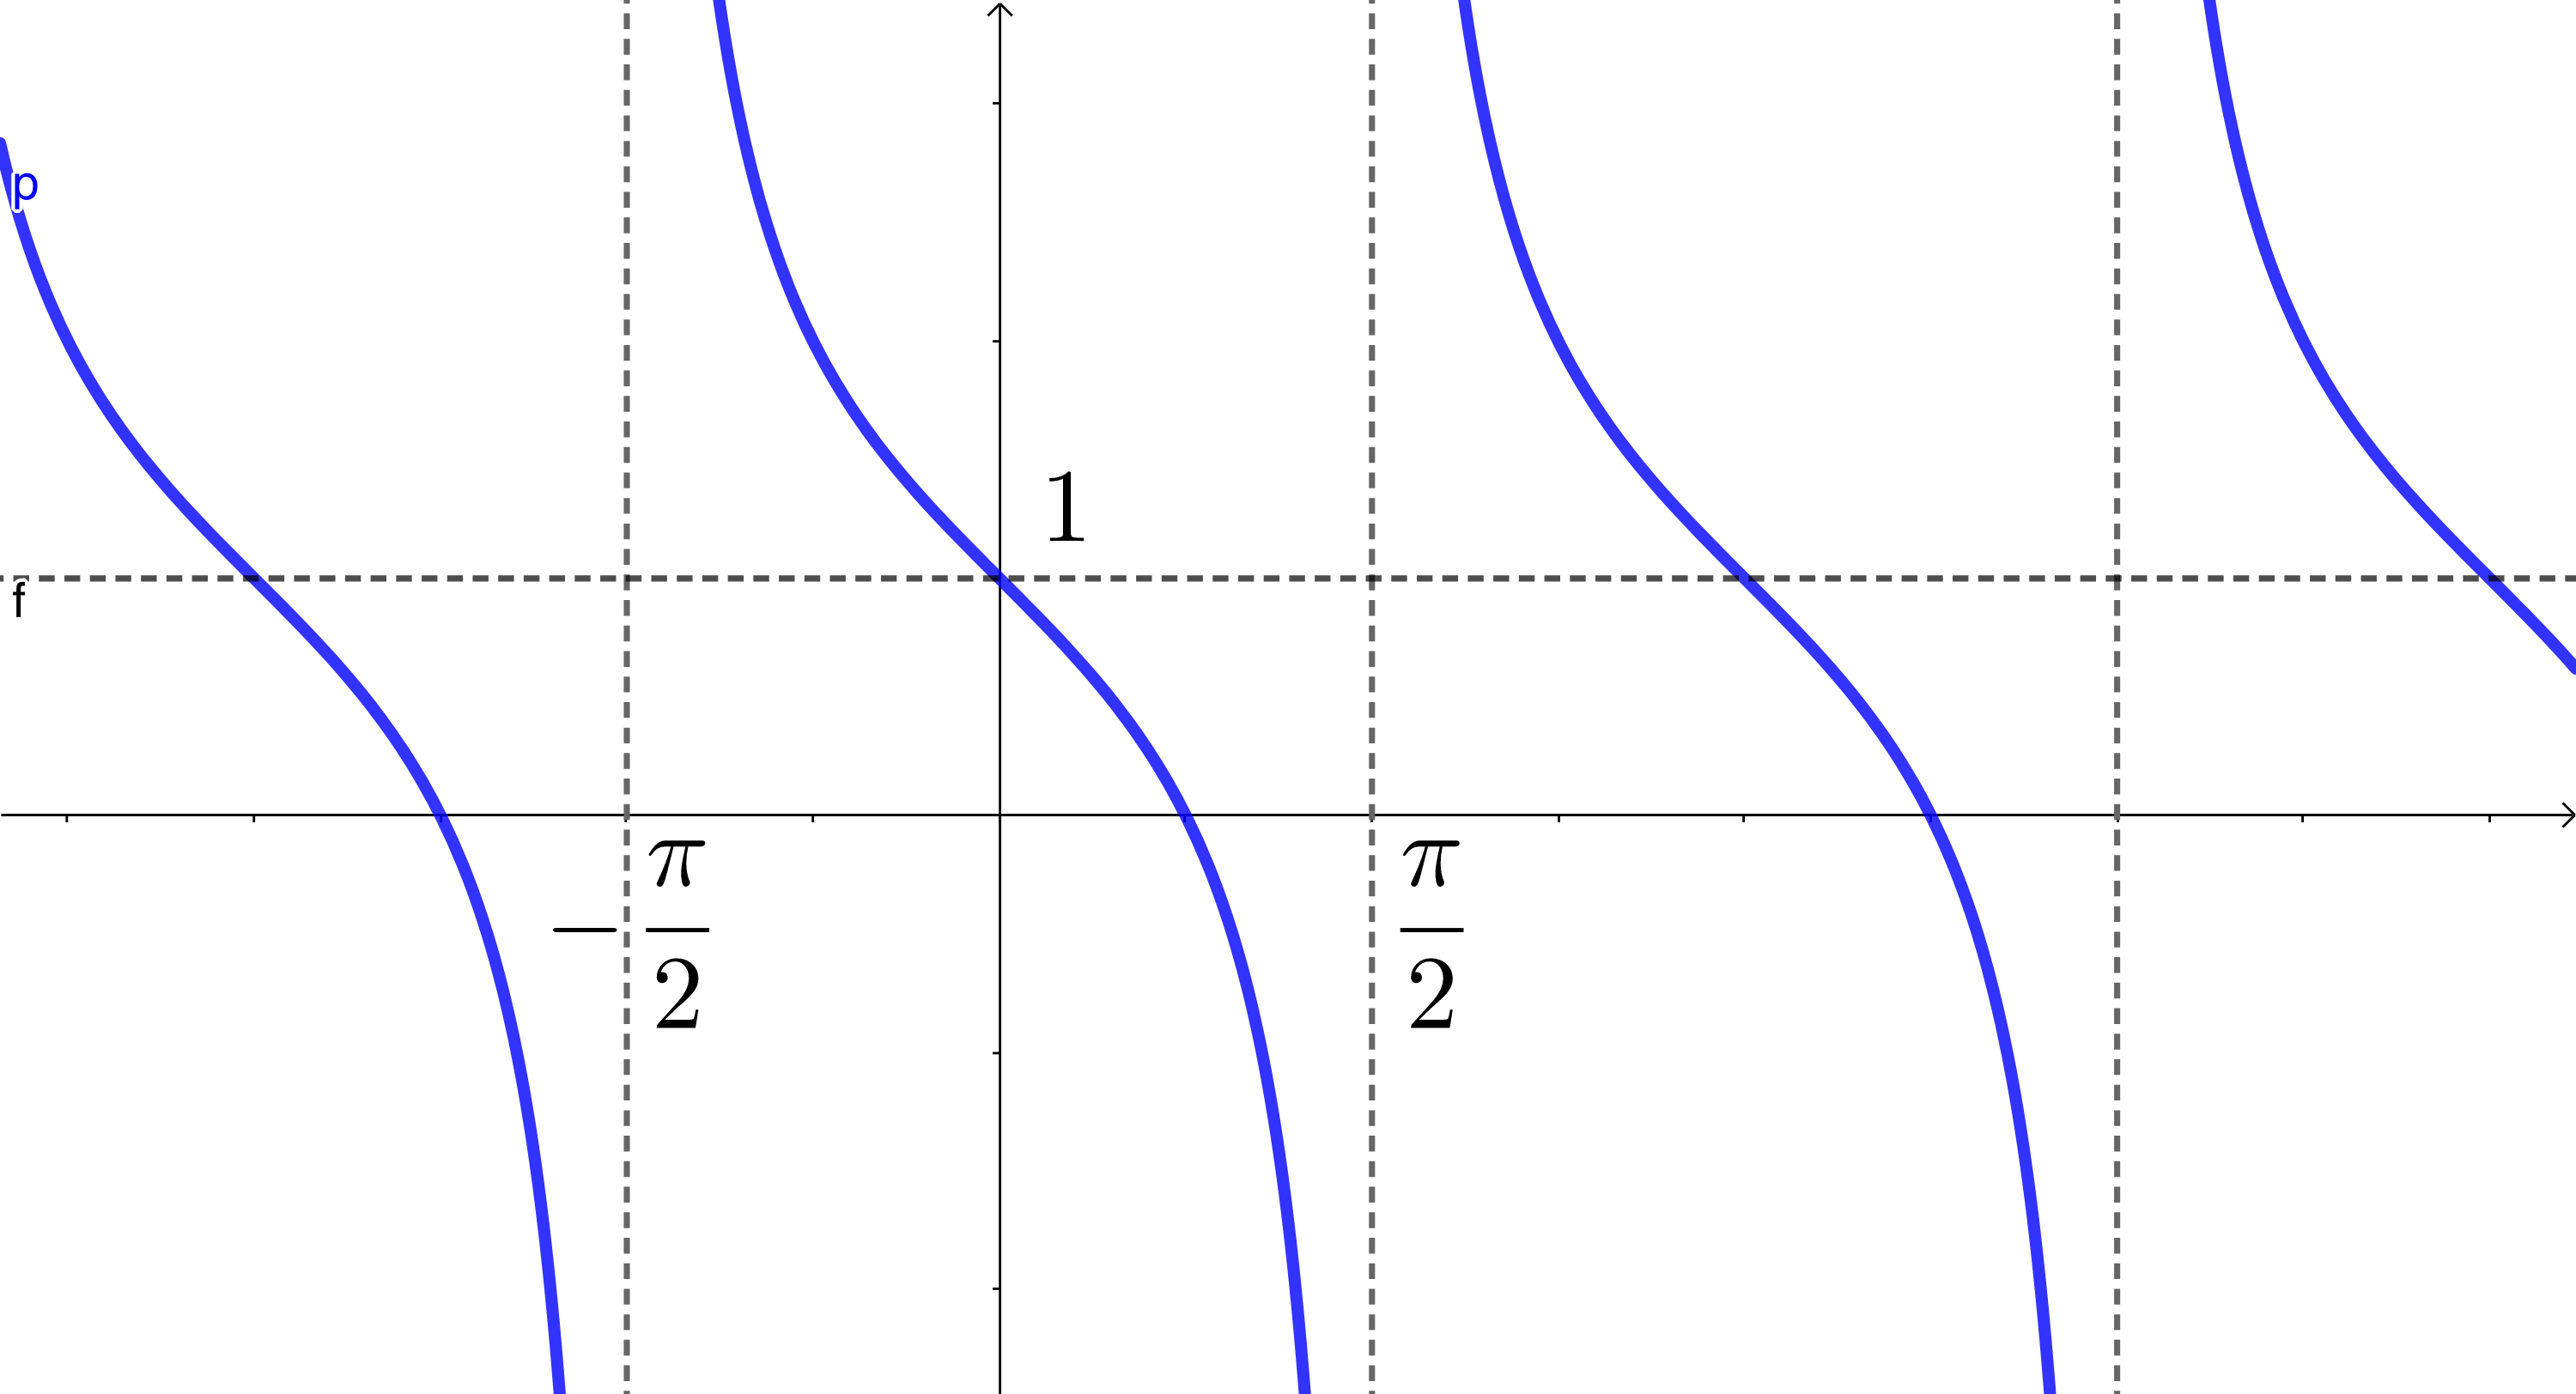
\includegraphics[width=6cm]{cap_trigon/figs/Grafico2.png}
        \vspace{.3cm}
        
        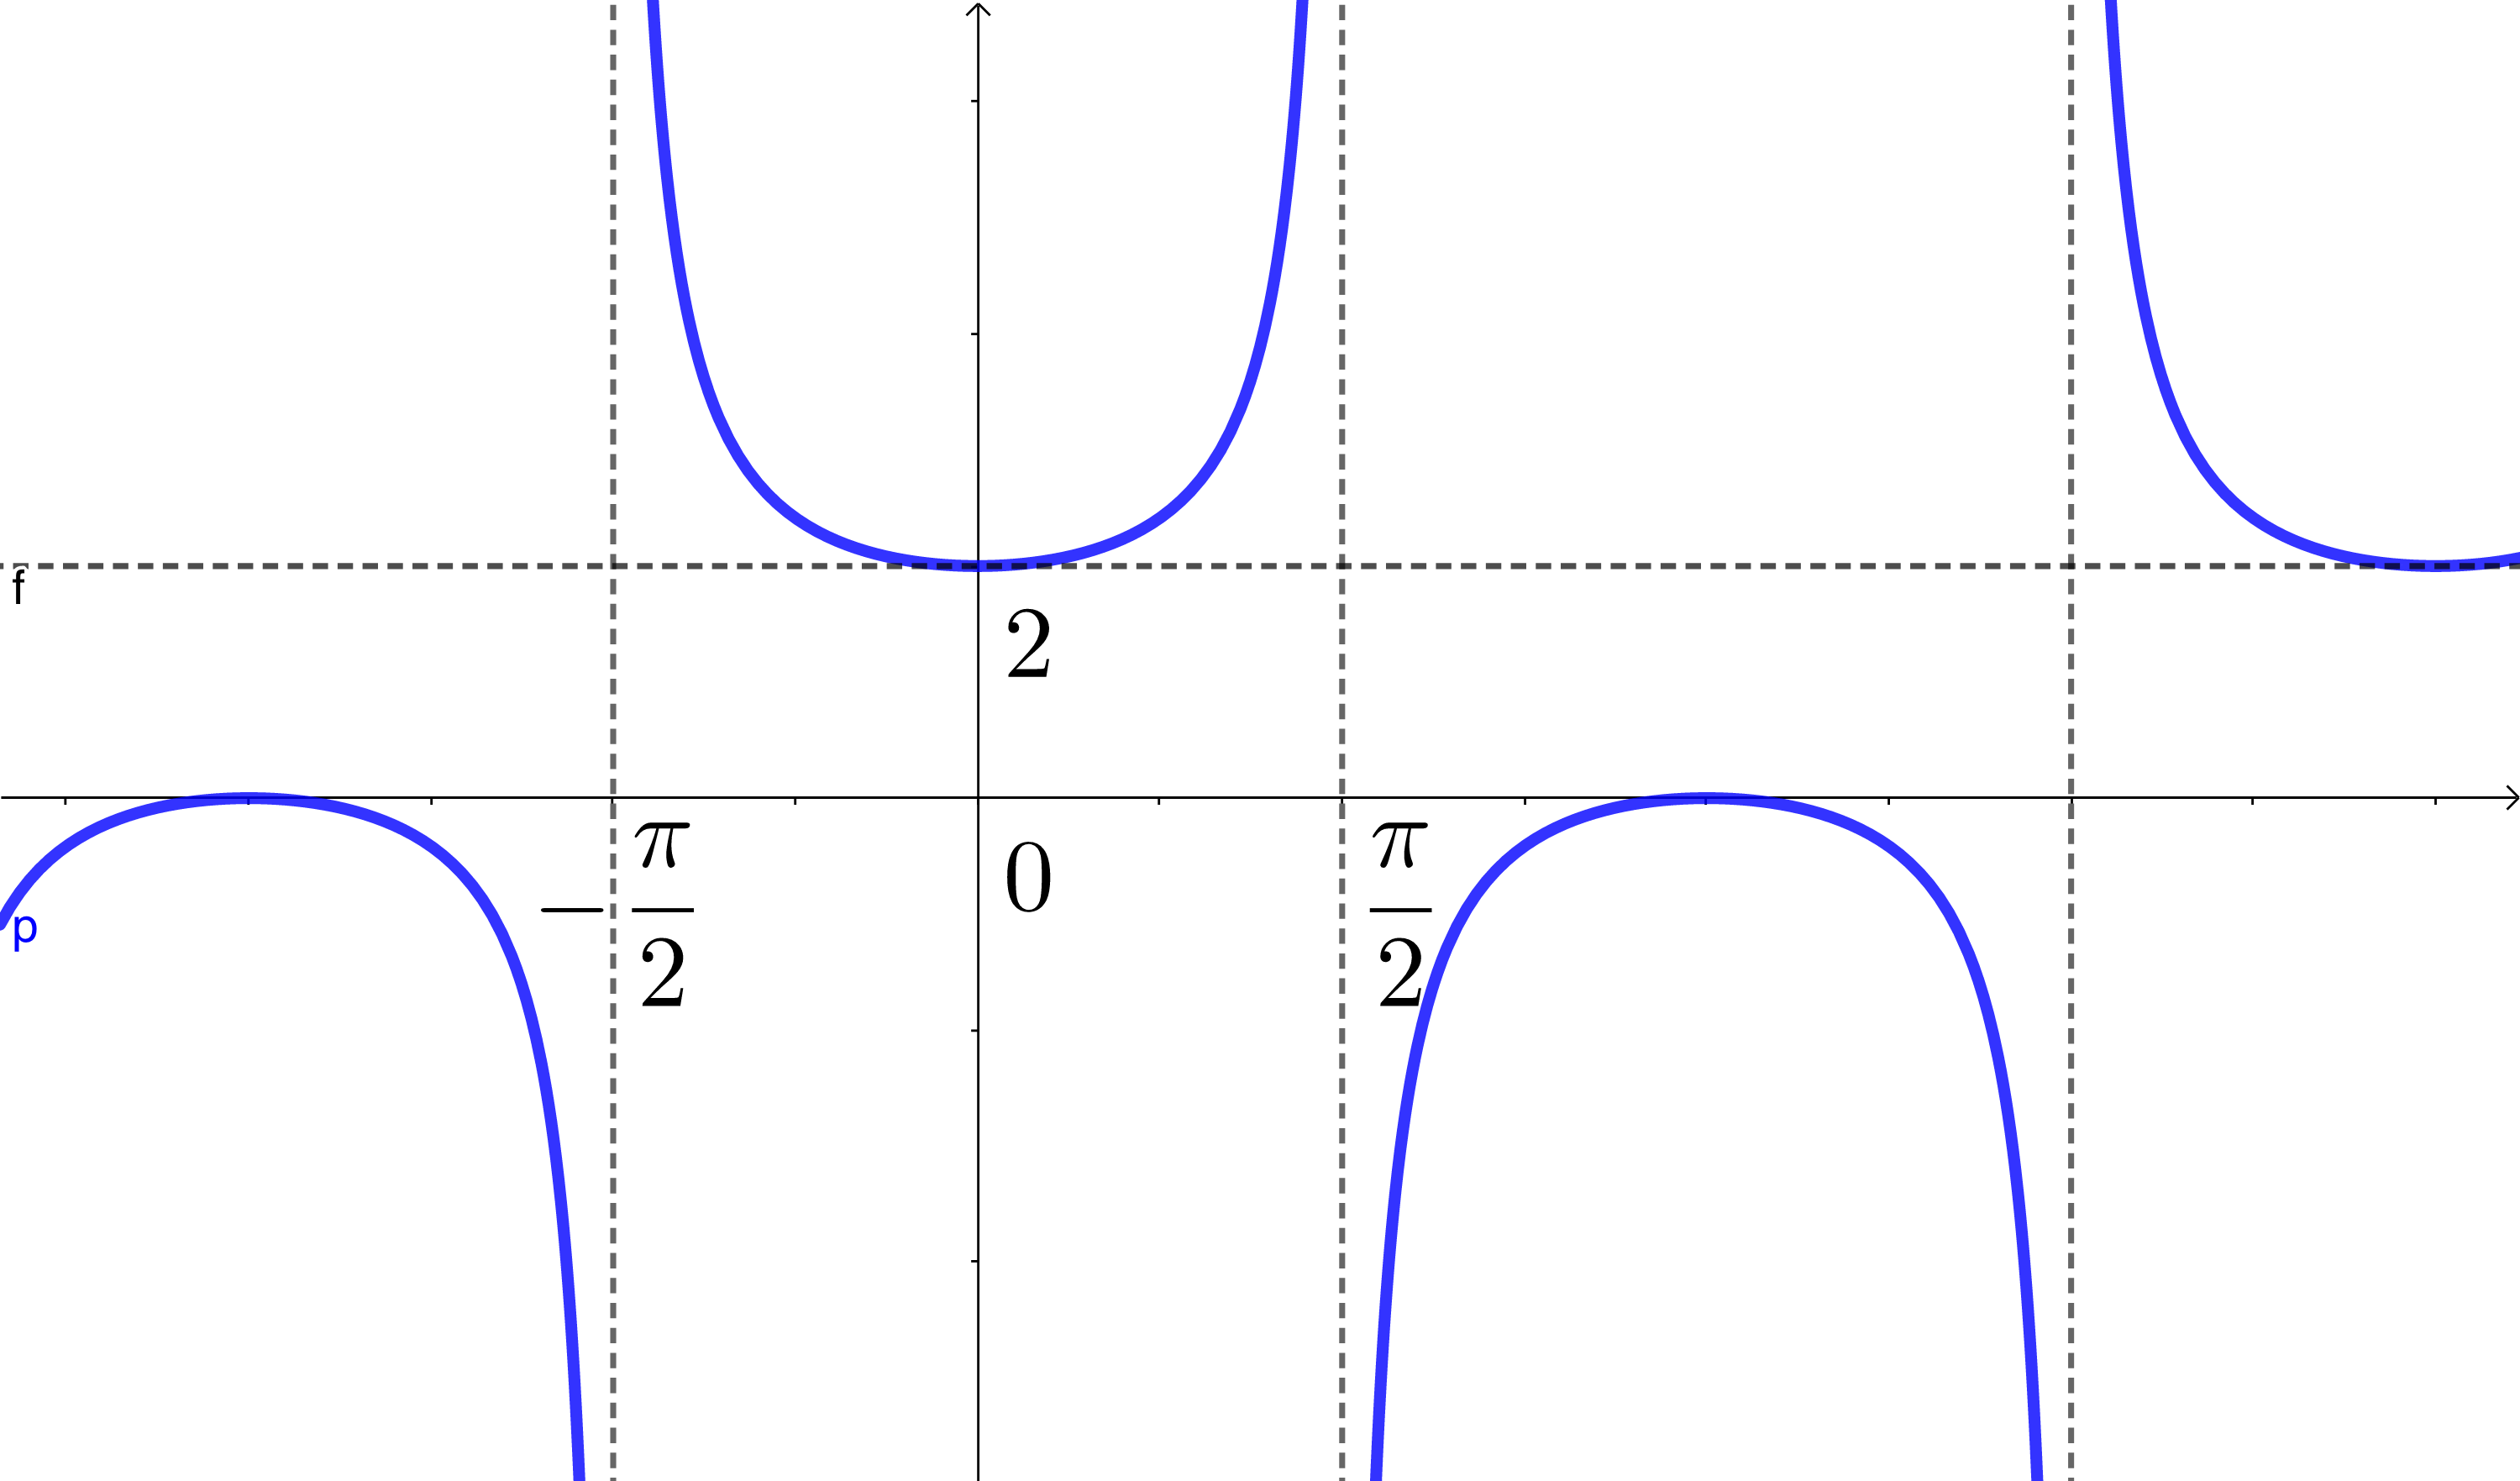
\includegraphics[width=6cm]{cap_trigon/figs/Grafico3.png}
    \end{center}
\end{exer}

\begin{exer}
     Exprima em função de $\sen x$ e $\cos x$ as expressões:
    \begin{enumerate}[a)]
        \item $\cos(5\pi +x)$
        \item $\cos(-\pi -x)$
        \item $\sen(\frac{5\pi}{2} +x)$
    \end{enumerate}
\end{exer}

\begin{exer}
    Qual o menor valor de $\dfrac{1}{3-\cos x}$, com $x$ real?
\end{exer}

\begin{exer}
    Se $\sec x=3$ e $\tg x<0$, determine o valor de $\sen x$.
\end{exer}

\begin{exer}
    Se $\sec x = \sqrt{3}$ e $\tg(x) < 0$, determine o valor de $\sen x$.
\end{exer}

\begin{exer}
    Suponha que $x$ é um arco no 3º quadrante tal que $\sec x = -\frac{4}{3}$. Calcule $\cotg(2x)$.
\end{exer}

\begin{exer}
    Se $\sen x = \frac{1}{3}$ e $\sec y= \frac{5}{4}$, onde $x$ e $y$ estão entre $0$ e $\frac{\pi}{2}$, calcule a expressão de:
    \begin{enumerate}[a)]
        \item $\sen(x+y)$
        \item $\cos(x-y)$
        \item $\sen(2y)$
    \end{enumerate}
\end{exer}


\begin{exer}
     Sendo $0\leqslant x < 2\pi$, resolva a equação $2\cos^2 x - \sen x -1 = 0$.
\end{exer}

\begin{exer}
Mostre que para qualquer número real $x$, temos
\begin{equation*}
    \sen\left(\frac{\pi}{3}+x\right)-\sen\left(\frac{\pi}{3}-x\right)=\sen x.
\end{equation*}
\end{exer}

\begin{exer}
    Verifique as seguintes identidades:
    \begin{enumerate}[a)]
        \item $\sen (2x)=2\sen x \cdot \cos x$
        \item $\cos(2x) = \cos^2 x- \sen^2 x$
        \item $\cos(\frac{\pi}{2}-x)=\sen x$
        \item $\sen(\pi - x)=\sen x$
        \item $\sen x \cdot \cotg x = \cos x$
        \item $\tg^2 x +\sen^2 x= \tg^2 x \cdot \sen^2 x$
    \end{enumerate}
\end{exer}

\begin{exer}
     Determine o valor $k$, para que exista o arco que satisfaz a igualdade
$$
\cos x = \dfrac{2k}{k+2}.
$$
\end{exer}

\begin{exer}
Calcule a seguinte identidade
$$\frac{2\tg x}{1+\tg^2 x}=\sen(2x).$$

Use isso para calcular o valor de $\tg15\degree$.
\end{exer}

\begin{exer}
Calcule a seguinte identidade
$$\cos(3x) = 4 \cos^{3} x - 3\cos x.$$

Use isso para verificar que $\cos 20^{\circ}$ é um zero do polinômio $p(x) = 8x^{3} -6x -1$.
\end{exer}



% \begin{exer}
%     Esboce o gráfico e determine a imagem e o período das funções a seguir:
%     \begin{enumerate}[a)]
%         \item $f(x)=\sen(7x-2)$
%         \item $f(x)=\sen(-2x+3)$
%         \item $f(x)=3+2\sen(2x-4)$
%         \item $f(x)=\cos(5x+1)$
%         \item $f(x)=5+3\cos(4x-7)$
%         \item $f(x)=\tg(3x+5)$
%         \item $f(x)=3+4\tg(-7x-5)$
%         \item $f(x)=\cotg(5x-1)$
%         \item $f(x)=3+4\cotg(7x-5)$
%         \item $f(x)=3+4\sec(5x-3)$
%         \item $f(x)=\cossec(-x-1)$
%         \item $f(x)=3-\cossec(3x-5)$
%     \end{enumerate}
% \end{exer}



%  \begin{exer}
%  Quando o Sol se encontra a $45\degree$ acima do horizonte, um poste de iluminação projeta sua sombra no chão com o comprimento de $12 m$. Determine a altura desse poste:
%  \end{exer}
% \begin{resp}
%   $12 m$
% \end{resp}

%  \begin{exer}
%  De acordo com o comandante e consultor técnico da ABEAR, Paulo Roberto Alonso, “o avião parte do solo em um ângulo de 15 graus, medida essa que vai reduzindo durante a subida”. Para facilitar nossos cálculos suponhamos que esta medida não se altere. Supondo que a região sobrevoada pelo avião seja plana, qual será a altura atingida pelo avião depois de percorrer $900 m$?
%  \end{exer}
% \begin{resp}
%   $\approx 232,9371 m$
% \end{resp}

%  \begin{exer}
%  Uma menina de $1,5m$ de altura avista o ponto mais alto de um morro, a partir de um ângulo de $20\degree$. Considerando que ela está a uma distância de $300m$ da base do morro, calcule a altura $(h)$ deste ponto.
%  \end{exer}
% \begin{resp}
%   $\approx 110,691 m$
% %    \par\noindent\rule{\columnwidth}{0.4pt}
% \end{resp}
\end{secExercicios}

%\subsection*{Respostas}

%\shipoutAnswer